\documentclass[../main.tex]{subfiles}

\begin{document}
\subsection{Functional Boxplots}
\label{sec:boxplots}

Only some of the previously described visualization methods work for continuous data and none of them can display multiple surface observations (e.g. multiple maps). One of the reasons it is so difficult to visualize conditional dependency in structurally complex datasets is due to the difficulty of even visualizing the probability distributions of these observations. 

\begin{figure}[H]
  \center
  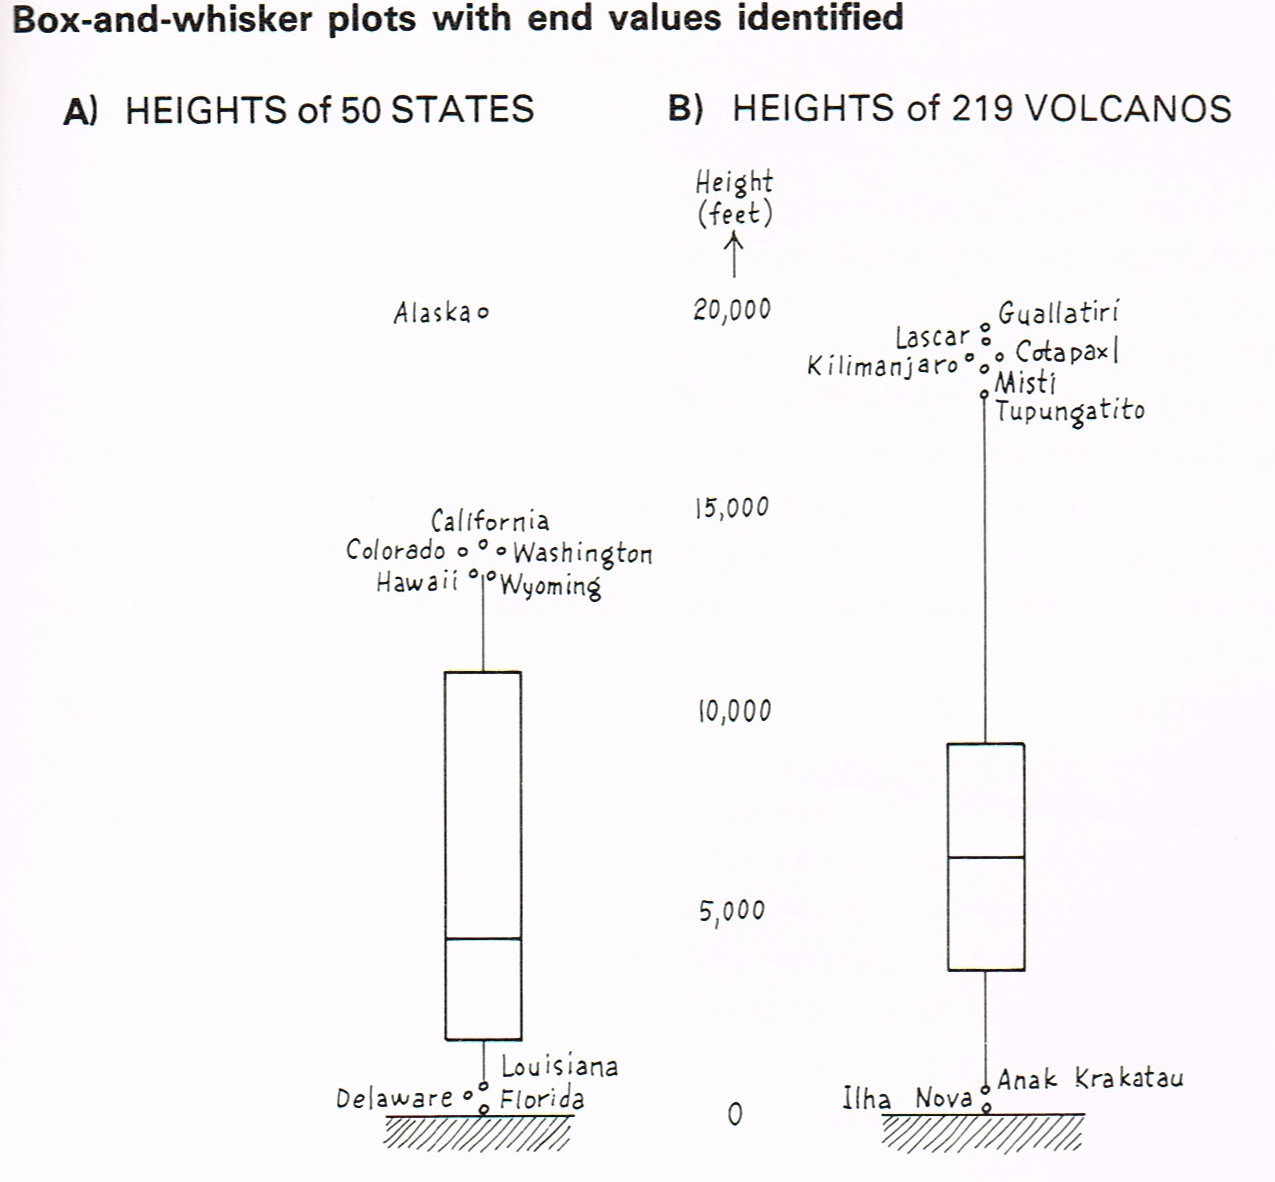
\includegraphics{boxplot}
  \caption{Tukey's 1977 example of the box plot shows the distribution of state and volcano elevations. The strength of the box and whisker is that it clearly shows that volcanoes tend to span a shorter range of average heights, but that the extremes are much further from the center. Figure is from \textit{Exploratory Data Analytics} \cite{tukey_exploratory_1977} }
  \label{fig:boxplot}
\end{figure}

The box plot is the standard method for visualizing the distribution of a quantitative variable and the box plot has evolved to display many more characteristics of the distribution \cite{wickham_40_2011}. Figure~\ref{fig:boxplot} illustrates that the distribution of volcano elevations is more densely packed at the center and has wider but leaner tails then the distribution of state elevations. While figure~\ref{fig:boxplot} shows the median, range between upper and lower interquartile, and lower and upper extreme \cite{tukey_exploratory_1977}, many authors have exploited the structure of the boxplot to encode more information. Authors used different quantile levels \cite{hyndman_sample_1996},xs or measures of outliers \cite{frigge_implementations_1989, schwertman_identifying_2007}, or otherwise incorporated skewness, kurtosis, and other descriptive distributional statistics \cite{kim_more_2004, marmolejo-ramos_shifting_2015}.

While box plots were designed to visualize discrete observations, there are methods for expanding them to functional observations. Understanding the distributions of functional observations requires ordering the functions such that there is some measure of how close these functions are to each other; traditional distance metrics discretize the observation into points sampled from the curve and so lose the overall structure of the curve. Instead functional observations are often ordered using band depth, which is the sum of the probabilities that the observations in any given functional observation fall within the max-min envelope defined by any two other functional observations \cite{Febrero_functional_2007,lopez-pintado_functional_2007}. Band depth and derivatives such as bivariate score depth \cite{rob_j._hyndman_rainbow_2010} and bivariate kernel density estimation \cite{scott_multivariate_1992} yield functional analogs to the median and other percentile metrics. For small values, the ordered curves can then be colored based on the ordering metric \cite{rob_j._hyndman_rainbow_2010}. 

\subsubsection{1D Curve}
\label{sec:curve}

\begin{figure}[H]
  \begin{subfigure}{\textwidth}
    \centering
    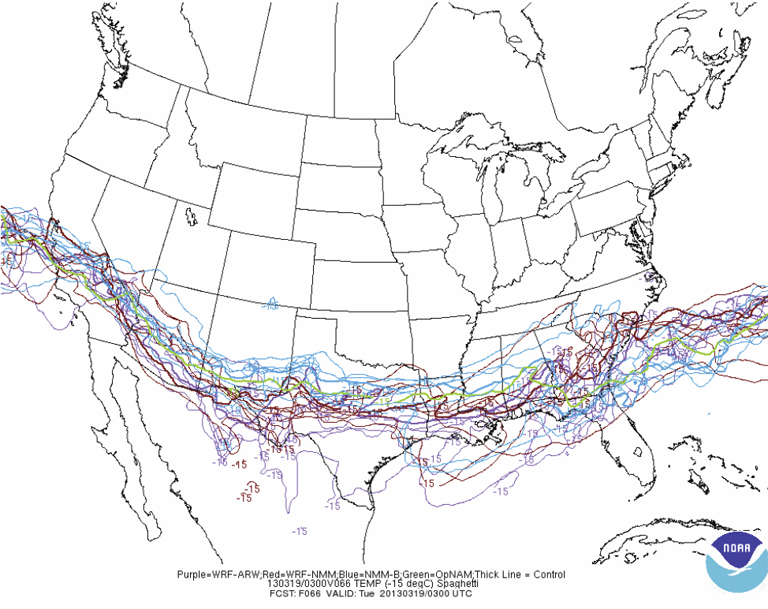
\includegraphics[scale=0.4]{spaghetti}
    \caption{Spaghetti plot of ensemble of 500mb -15C temperature isocountours.}
    \label{fig:spaghetti}
    \end{subfigure}

    \bigskip
    \begin{subfigure}{\textwidth}
    \centering
    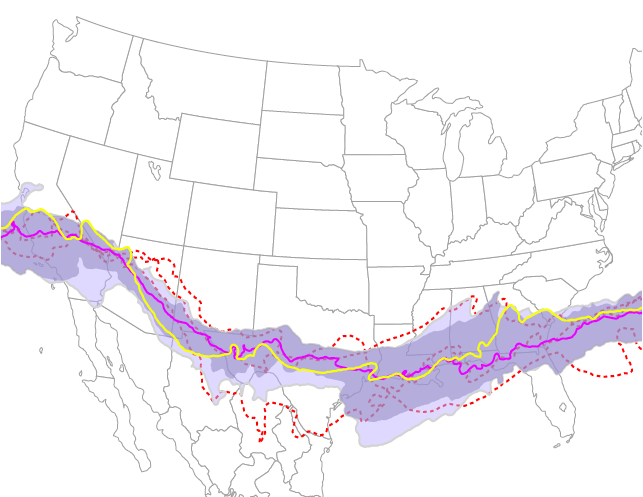
\includegraphics[scale=0.5]{contour_weather}
    \caption{Contour boxplot showing the distribution of a 500mb -15C temperature field. The mean field is in yellow, the median in purple, and the dashed red lines are the outlier cut off bands.}
    \label{fig:contour}
    \end{subfigure}

    \caption{Figures are from \textit{Contour boxplots: A method for characterizing uncertainty in feature sets from simulation ensembles} \cite{whitaker_contour_2013}}
\end{figure}

Climate and weather models are functional, and increasingly they are ensembles of models with slightly different parameters; to analyze the skill of these models, it is important to visualize the spread in the predictions of the ensemble members. Functional bag, box, and HDR plots \cite{rob_j._hyndman_rainbow_2010, sun_functional_2011} can all be used to show the distribution of ensemble predictions, but contour box plots \cite{whitaker_contour_2013} are designed to highlight the variability in the predictions. In figure~\ref{fig:contour}, the ensemble members are ordered by band depth such that the median band is the ensemble member with about 50\% of its members within all envelopes formed by the other bands. As illustrated by figure~\ref{fig:contour}, the contour boxplots are an improvement over the spaghetti  plots \cite{luo_visualizing_2003, whitaker_contour_2013} in figure~\ref{fig:spaghetti} because the authors replace most of the bands with an outlying envelope in light purple-gray and a more central envelope in darker purple-gray. The contour boxplot effectively displays variability in isocountour data, but is also inherently limited to curves.

\subsubsection{2D Surface}
\label{sec:surface}
\begin{figure}[H]
  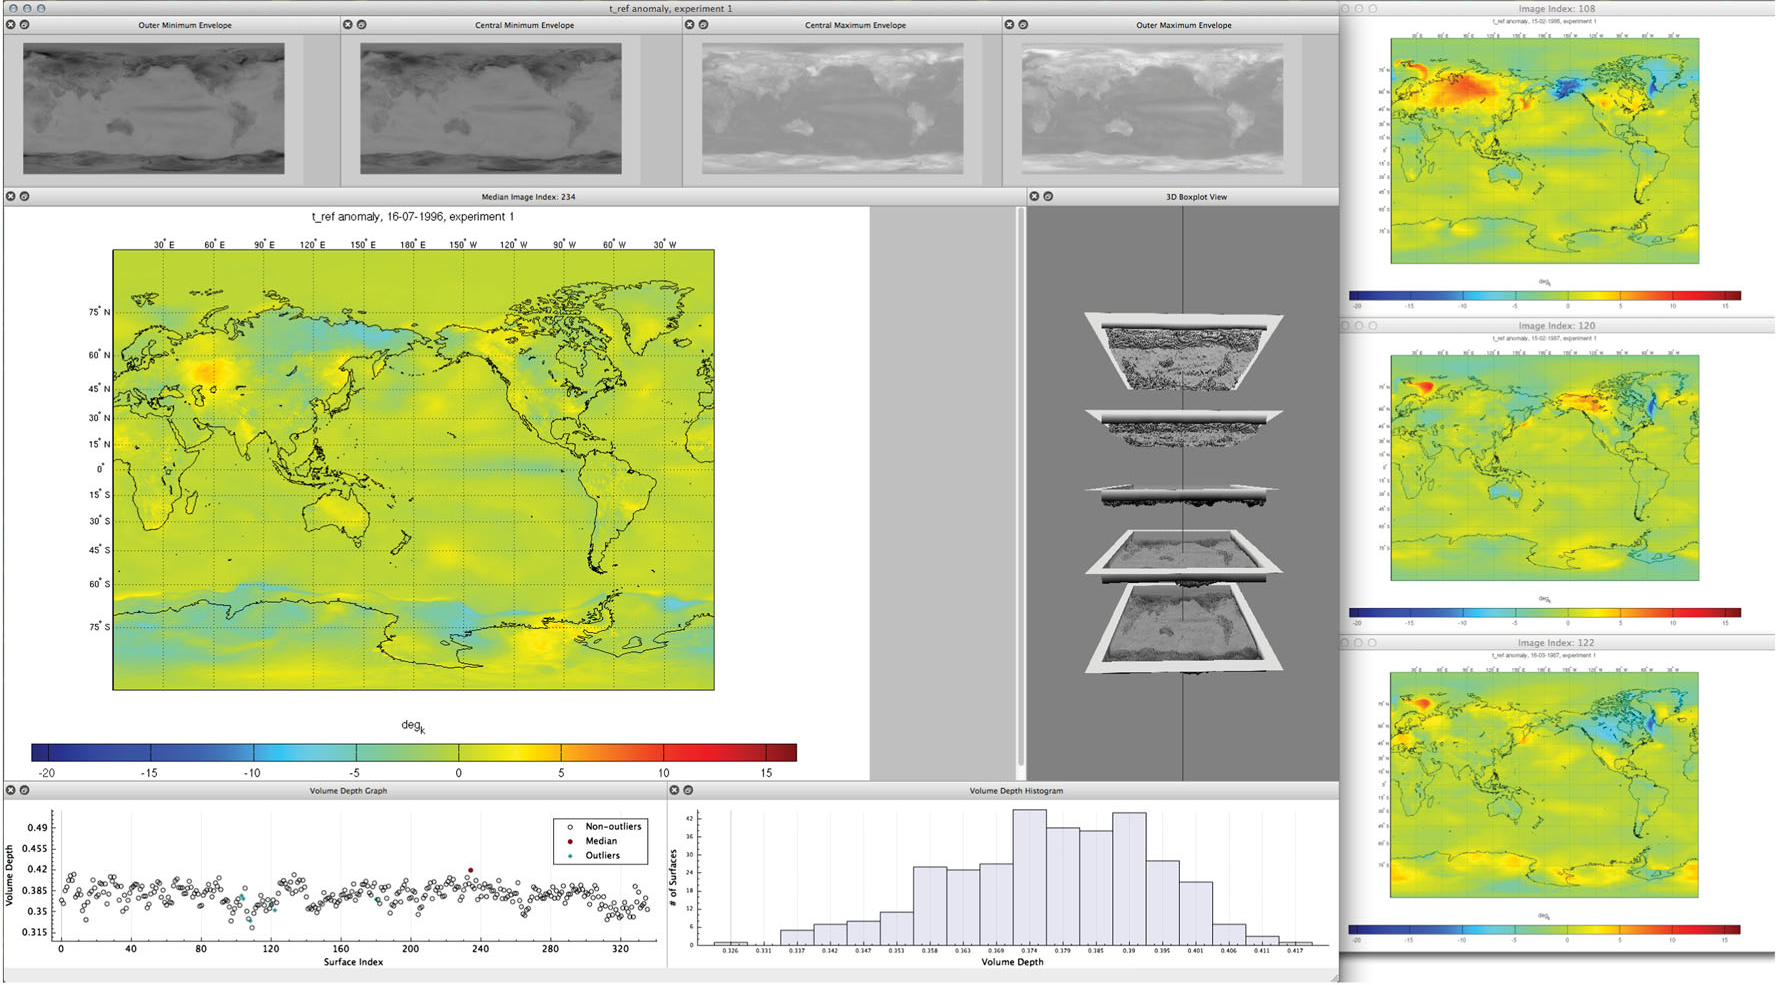
\includegraphics[width=1\linewidth]{surfacebox.png}
  \caption{The large colored heatmap in the middle of the dashboard is the median surface. The surfaces at the top of the dashboard are minimum and maximum envelopes. The graphs at the bottom visualize the distribution of the band-depths of the surfaces. The 3 surfaces on the right are outliers. This figure is from \textit{Surface boxplots} \cite{genton_surface_2014}}
  \label{fig:surface}
\end{figure}

Functional climate and weather models are often regional or global, and it is just as critical to understand the spatial distribution of predictions as the temporal ones. In figure~\ref{fig:surface}, Genton et al. built a surface boxplot visualization tool with multiple panes \cite{genton_surface_2014}. Like a traditional boxplot, the surface boxplot tools displays the median surface and minimum and maximum surfaces. The tool also provides a 3D view of how the surfaces are distributed. Like many other functional boxplot methods, the surfaces are ordered using the band depth metric; therefore the tool also visualizes the distribution of the surface band-depths. As with the functional and contour boxplots (\ref{sec:curve}), the surface boxplot is overly specific to data that is a series of surfaces. 
\end{document}